\documentclass[10pt,a4paper]{amsart}
\usepackage[margin=19mm]{geometry}
\usepackage{amsmath,amssymb,mathtools}
\usepackage[scr=rsfs,cal=euler]{mathalfa}
\usepackage{xfrac}
\usepackage[unicode,hidelinks,bookmarks=false]{hyperref}
\newcommand{\ie}{i.e.\ }
\newcommand{\cf}{cf.\ }
\newcommand{\resp}{respectively\ }
\newcommand{\Subsection}{\subsection}
\providecommand{\nobreakdash}{\nobreak\hbox{-}}
\setlength{\emergencystretch}{2em}
\multlinegap0pt
\usepackage{tikz}
\usepackage{xcolor}
\usepackage{amssymb}
\usepackage{mathtools}
\usepackage{bm}
\usepackage{float}
\usepackage{csquotes}
\newtheorem{theorem}{Theorem}
\usepackage{cleveref}
\crefname{theorem}{Theorem}{Theorems}
\title{Balanced Spanning Trees for Triangular Strip Lattices}
\author{Saugat Dhakal, Long Nguyen, Yandi Wu}
\date{Source: arXiv:2609.08222v1 (CC BY 4.0)}
\begin{document}
\maketitle

\noindent\emph{Source and licence.} Balanced Spanning Trees for Triangular Strip Lattices. Version arXiv:2609.08222v1 (CC BY 4.0), distributed by arXiv under the Creative Commons Attribution 4.0 International licence, http://creativecommons.org/licenses/by/4.0/, as recorded in the arXiv licence metadata for this exact version and shown on the abstract page https://arxiv.org/abs/2609.08222v1. Full licence notice: \texttt{licenses/arxiv-2609.08222-CC-BY-4.0.txt}.\par\smallskip

\noindent\textit{Editorial scope.} Counted unit: the article's theorem thm:sthomogenousodd (source0.tex lines 578--582). The article's complete original proof of it is delivered with it (source0.tex lines 583--656, one \texttt{proof} environment of 74 lines). No mathematics is written, repaired or re-derived: the statement and the proof are the article's own lines, in the article's own notation, and no retained line is substituted or re-flowed.  Retained uncounted as the source-local context the proof needs: lines 523--528; lines 531--537.  Nothing was omitted from any retained span, so the package carries no omission record.  No retained line contains a citation, so the wrapper carries no bibliography and no bibliography entry.  The retained lines contain the article's own diagram code, which the wrapper typesets with the standard tikz packages; no image file is delivered and the package declares no asset dependency.  Editorial formatting only, in addition: an AMS \texttt{amsart} preamble that restates the article's own declarations and macros used by the retained lines, namely the environments \texttt{theorem} on separate counters, together with the standard packages those lines need.  The retained environments print in this document as Theorem 1 in order of appearance, whereas the article prints the same items with the numbering of its own full document.  The complete native source of the article as distributed in the arXiv e-print for this exact version is bundled unchanged as \texttt{sources/209704/source0.tex}.
\begin{equation}\label{eqn:recurrencerelationspanningtree} 
    \begin{aligned}
    T_{2(n+2)} = 7T_{2(n+1)} - T_{2n},\\
    \text{ and } F_{2(n+2)} = 7F_{2(n+1)} - F_{2n}.
    \end{aligned}
\end{equation}

\begin{equation}\label{eqn:initialvalues1}
    \begin{aligned}
    T_2 = 1, \quad T_4 = 8,\\
    \quad \text{and} \quad
    F_2 = 1, \quad F_4 = 5.
    \end{aligned}
\end{equation}

\begin{theorem}[Number of spanning trees in $\Gamma_{2n - 1}$]\label{thm:sthomogenousodd}
The number of spanning trees in $\Gamma_{2n - 1}$, denoted by $T_{2n - 1}$ satisfies the recurrence relation: 
\[\ T_{2n+3} = 7T_{2n+1} - T_{2n - 1}.\]
with initial conditions $T_3 = 3$ and $T_5 = 21.$
\end{theorem}

\begin{proof} 
    \par %Since, the diagonal edge is predetermined by the structure of $\Gamma_{2k - 1}$, we only consider one of the two possible diagonals, the one that goes from the top left to the bottom right. Even if the diagonal determined by $\Gamma_{2k - 1}$ is the other diagonal, it doesn't affect our count of the spanning trees.
    Since the orientation of the diagonal edge is determined by the structure of $\Gamma_{2k-1}$, we may assume without loss of generality that the diagonal joins the upper-left and lower-right vertices. The opposite orientation is symmetric and therefore yields the same number of spanning trees.
    \par
    Now, we follow the counting technique as the one presented in the last section with some minor changes. We also use the recurrence relation established in the last section to make our work easier. As before, we denote the rightmost vertices of $\Gamma_{2(n - 1)}$ by $\{u, v\}$. To get a spanning tree in $\Gamma_{2n - 1}$, we can either expand from a spanning tree in $\Gamma_{2(n - 1)}$ or expand from a forest in $\Gamma_{2(n - 1)}$ consisting of two trees each containing a distinct vertex in $\{u, v\}$. Observe from \Cref{fig:R_{2n - 1}} that there are only two ways to get a spanning tree in $\Gamma_{2n - 1}$ from a spanning tree in $\Gamma_{2(n - 1)}$ and only one way  from a forest in $\Gamma_{2(n - 1)}$.


    \begin{figure}[htbp]
        \centering
        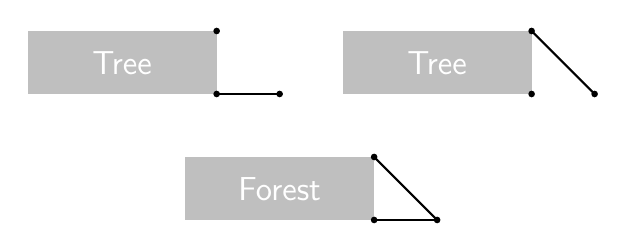
\begin{tikzpicture}[thick, every node/.style={font=\sffamily\large},xscale=0.8,yscale=0.8]
    %\draw[help lines] grid(9,3);
    % -------------------------
    % Top Left Graph ("Tree")
    % -------------------------
    \fill[lightgray] (0, 2) rectangle (3, 3);
    \node at (1.5, 2.5) {\textcolor{white}{Tree}};
    
    
    % Dots on the right edge
    \fill (3, 3) circle (1.5pt);
    \fill (3, 2) circle (1.5pt);
    
    % Horizontal extension from bottom corner
    \draw (3, 2) -- (4, 2);
    \fill (4, 2) circle (1.5pt);

    % -------------------------
    % Top Right Graph ("Tree")
    % -------------------------
    \fill[lightgray] (5, 2) rectangle (8, 3);
    \node at (6.5, 2.5) {\textcolor{white}{Tree}};
    
    % Dots on the right edge
    \fill (8, 3) circle (1.5pt);
    \fill (8, 2) circle (1.5pt);
    
    % Diagonal extension from top corner
    \draw (8, 3) -- (9, 2);
    \fill (9, 2) circle (1.5pt);

    % -------------------------
    % Bottom Graph ("forest")
    % -------------------------
    \fill[lightgray] (2.5, 0) rectangle (5.5, 1);
    \node at (4, 0.5) {\textcolor{white}{Forest}};
    
    % Dots on the right edge
    \fill (5.5, 1) circle (1.5pt);
    \fill (5.5, 0) circle (1.5pt);
    
    % Extension forming a triangle on the right
    \draw (5.5, 1) -- (6.5, 0);
    \draw (5.5, 0) -- (6.5, 0);
    \fill (6.5, 0) circle (1.5pt);

\end{tikzpicture}
        \caption{The possible ways to obtain a spanning tree in $\Gamma_{2n - 1}$.}
        \label{fig:R_{2n - 1}}
    \end{figure}
    \par
    So, from this, we obtain the following recurrence relation: 
    \[ T_{2n + 1} = 2T_{2n} + F_{2n}.\]
    
    Using the recurrence relation from (\ref{eqn:recurrencerelationspanningtree}) and making the appropriate substitutions, we get the following: 
    \begin{equation} \label{eqn:recurrencerelationspanningtreeodd} 
     T_{2n+3} = 7T_{2n+1} - T_{2n-1}
 \end{equation}
    Also, from (\ref{eqn:initialvalues1}), we can find the initial values $T_3$ and $T_5$.
    \begin{equation}\label{eqn:initialvalues2}
    T_3 = 2T_2 + F_2 = 2(1) + 1 = 3
    \quad \text{and} \quad
    T_5 = 2T_4 + F_4 = 2(8) + 5 = 21,
\end{equation} which completes our proof.
\end{proof}

\end{document}
